\chapter{Reproducibility}
This chapter describes the source code repository and provides the information and  instructions of how to use, alter and/or improve the current version of the Hop-by-hop measurement framework. 

\section{The Source Code Repository}
The source code repository for this thesis is located on the GitLab instance belonging to the TUM. The \texttt{ma-andguladze/App} directory contains the whole source code.

The tool consists of the following files:
\begin{itemize}
  \item \texttt{PPrate.py} - The pprate algorithm implementation by Patryk Brzoza\cite{Brzoza}
  \item \texttt{TrafficGenerator.c} - As the name suggests, this program generates TCP traffic from one host to another. It takes the IP addresses of two hosts as arguments and creates the traffic via raw sockets. The file should be compiled before the first run.
  \item \texttt{mininet\textunderscore topo.py} - Builds an instance of the network in Mininet considering all the necessary parameters passed, conducts the traffic generation, captures the traffic and saves the results in pcap files.
  \item \texttt{prepare\textunderscore test.py} - Contains several helper functions, most notably the config file parser and the capacity generator.
  \item \texttt{process\textunderscore tcp\textunderscore csv.py} - Converts the Calculates the end-to-end capacity of the network. Implementation by Brzoza\cite{Brzoza}
  \item \texttt{process\textunderscore icmp\textunderscore csv.py} - Converts the \texttt{icmp.pcap} file into csv and delivers the hop-by-hop capacity estimations based on the latter 
  \item \texttt{run\textunderscore test.py} - The main file that bootstraps the tool and runs the experiments in one setting. It requires a \texttt{JSON} configuration file to be passed as an argument with the help of which it is possible to manipulate several key parameters necessary for testing.
\end{itemize}

\begin{figure}[htp]
 \centering
 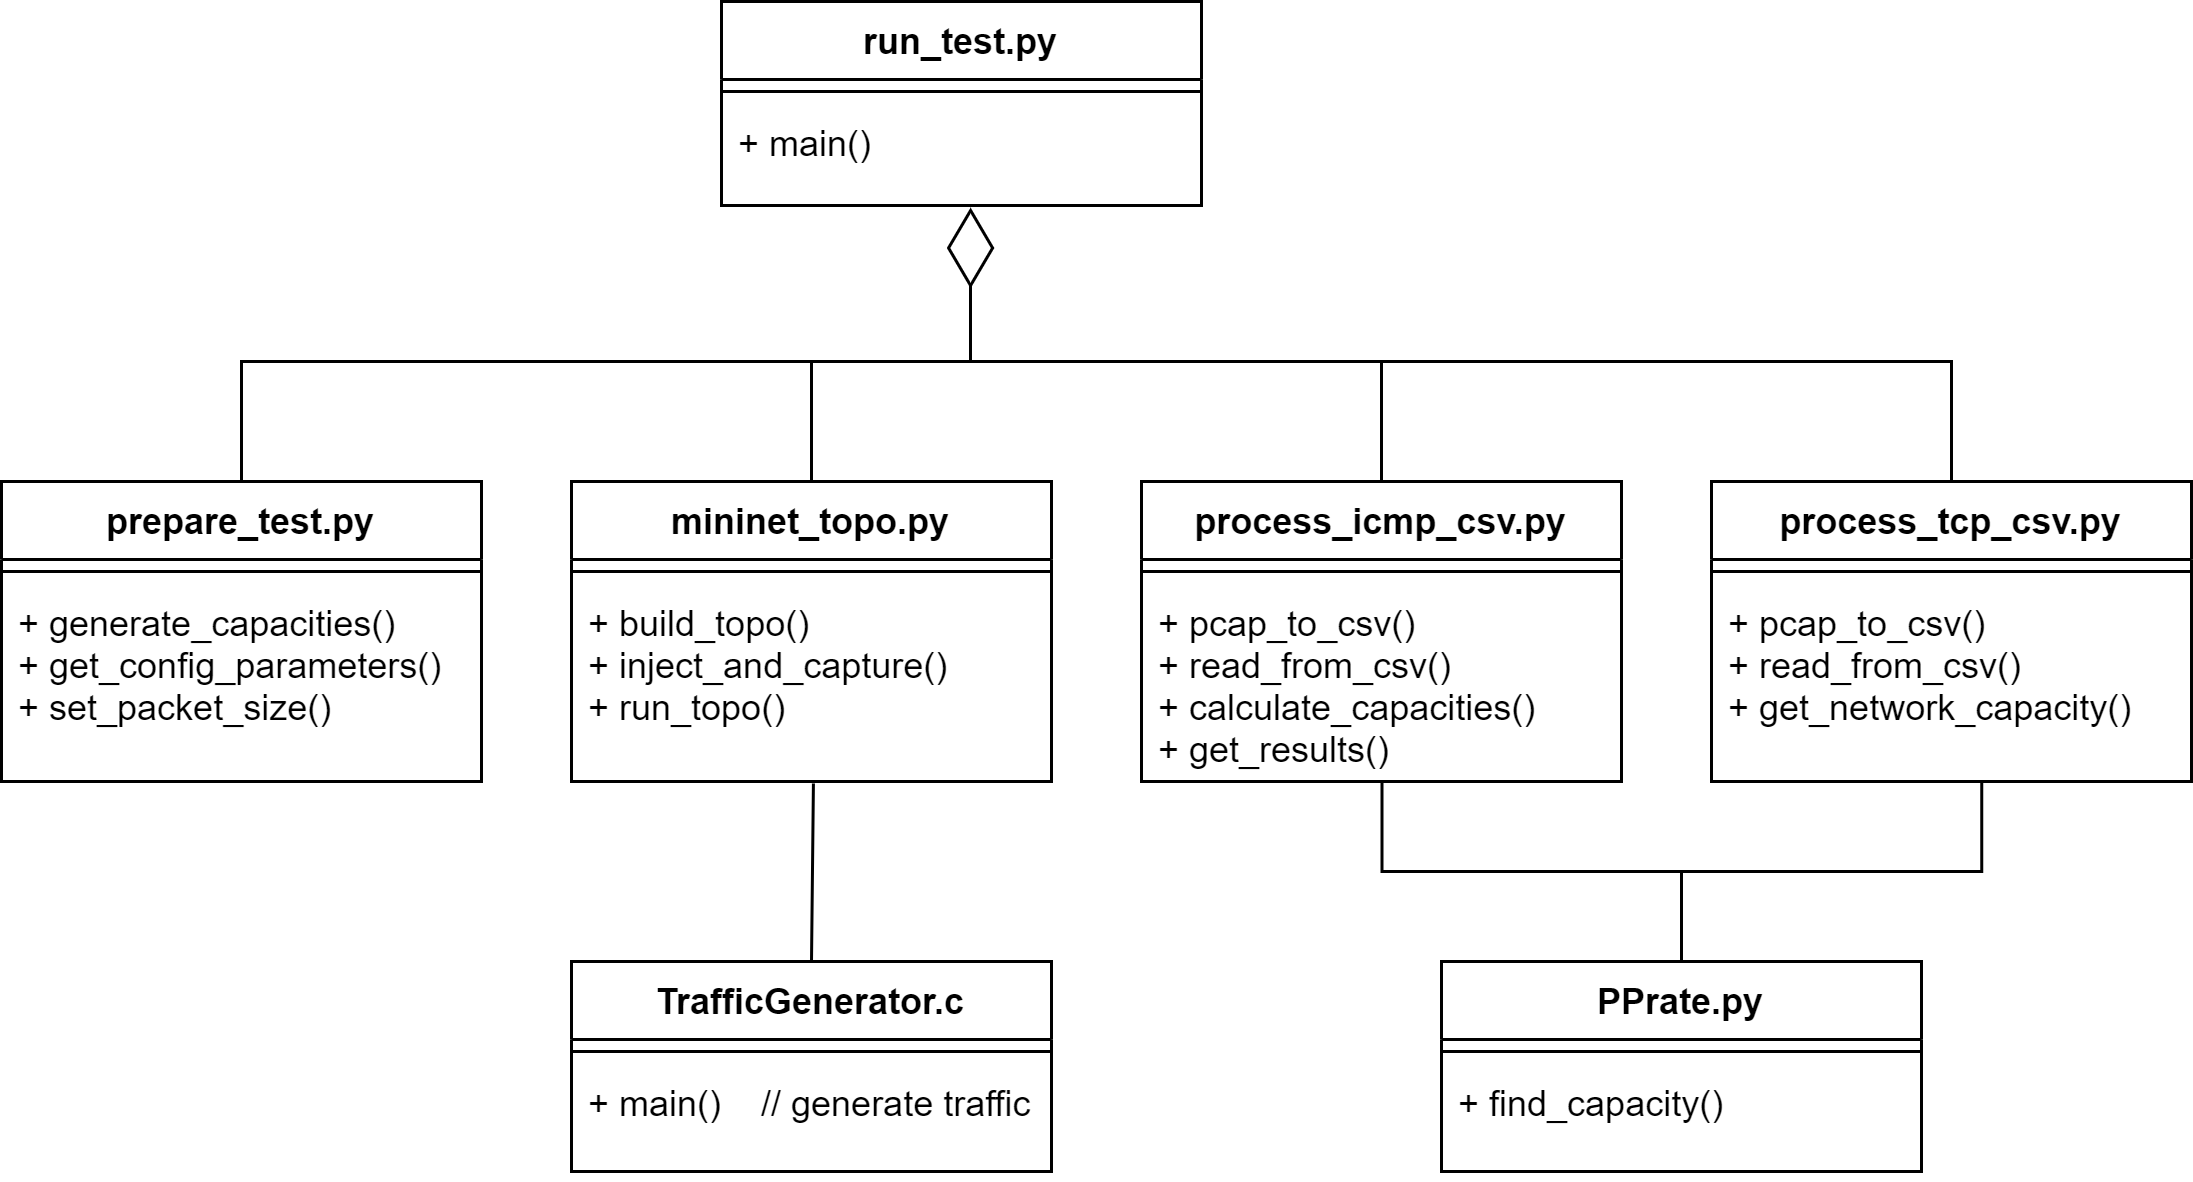
\includegraphics[width=\textwidth]{architecture}
 \caption{The architecture of the framework}
 \label{architecture}

\end{figure}


\section{Setup}
In order to run the test measurements with our tool, several dependencies and software should be installed on the Linux machine.

The experiments conducted by us were run only on Mininet - a network emulator tool which creates a realistic virtual network of virtual hosts, switches, controllers and links and runs a real kernel and application code\cite{mnHome}.
To run the experiments on Mininet, it is necessary to install the emulator first.
It is highly recommended to install Mininet from the source GitHub repository instead of packages, as the Mininet homepage\cite{mnInstall} states that packages could give an older version. 

Mininet installation:
\begin{lstlisting}[language=bash]
  $ git clone git://github.com/mininet/mininet
  $ mininet/util/install.sh [options]
\end{lstlisting}
The default branch normally will install the latest stable version, however in case a user wishes to have any other version, it also possible to check out the branch with the following script before running \texttt{install.sh}:
\begin{lstlisting}[language=bash]
  $ cd mininet
  $ git tag  # list available versions
  $ git checkout -b mininet-2.3.0 2.3.0  # or any desired version from the list
  $ cd ..
\end{lstlisting}
\emph{Note that Mininet must run as a root.}


As for the rest, the following dependencies are required to be installed to run experiments:
\begin{itemize}
	\item pandas
	\item NumPy
	\item SciPy
	\item tshark
	\item iPerf
\end{itemize}
For setting up these and compiling the \texttt{TrafficGenerator.c} program, run \texttt{install.sh} script in the \texttt{ma-andguladze/App} directory.

\section{Running Tests}
The measurements must be run with a \texttt{JSON} config file containing all the parameters that are interesting and important for our measurements. Manipulating these parameters gives us a better picture about strengths and weaknesses of our approach.

The following script executes the experiment:
\begin{lstlisting}[language=bash]
  $ sudo python run_test.py config.json
\end{lstlisting}

The following \texttt{JSON} serves as an example of a configuration file used for experiments.
It contains default parameter values, each of which will be manipulated respectively in upcoming sections:
\begin{lstlisting}
{    
  "topo_size": 3, // path length
  "capacity_range": [10, 100],			
  "capacity_delta": 5
  "packet_size": 1400,
  "packets_per_hop": 300,
  "icmp_ratelimit": 0,
  "packet_loss": 0,
  "cross_traffic": 0.0,
  "output": "results/results.csv"
}
\end{lstlisting}

\textit{\textbf{Disclaimer:} \texttt{packet\textunderscore loss} is a probability, therefore it does not always cause the packet loss during test runs; On the other hand, regular test runs with \texttt{packet\textunderscore loss = 0} can result in lost packets.}
